\documentclass[11pt,a4paper]{article}
\usepackage{wok-editorial}

\begin{document}

\woktitle{DNA}{WOK}{Maio 2026}{Programação Dinâmica, Strings}

\begin{objetivobox}
\textbf{Objetivos Pedagógicos:}
\begin{itemize}
    \item Desenvolver proficiência na clássica técnica de Programação Dinâmica bi-dimensional (LCS - Longest Common Subsequence).
    \item Entender como adicionar restrições condicionais baseadas em estados contínuos (tamanho mínimo de bloco).
    \item Aprender a otimizar a transição de estado da DP de $O(N^3)$ para $O(N^2)$ usando vetores auxiliares.
\end{itemize}
\end{objetivobox}

\section*{Disciplinas Relacionadas}

\begin{table}[h]
\centering
\begin{tabularx}{\textwidth}{|l|X|}
\hline
\textbf{Disciplina} & \textbf{Tópico Aplicado} \\
\hline
Algoritmos e Estruturas de Dados II & Programação Dinâmica e Processamento de Strings (Bioinformática). \\
\hline
Análise de Complexidade & Redução do custo da função de transição de $O(N)$ para $O(1)$ constante em cada célula. \\
\hline
Lógica Matemática & Avaliação de subproblemas ótimos e independência de blocos de prefixo. \\
\hline
\end{tabularx}
\end{table}

\tagcloud{Programação Dinâmica, DP 2D, Bioinformática, Blocos Contíguos, Otimização O(N\textsuperscript{2})}

\section*{Editorial Completo}

Neste problema, o desafio central não é apenas encontrar a maior subsequência em comum (como no clássico LCS), mas sim impor que as letras escolhidas devem compor \textbf{segmentos contínuos de no mínimo tamanho $K$}.

A abordagem inocente seria, a cada célula $(i,j)$ de uma matriz padrão, varrer um contador $c$ de $K$ até o número máximo de combinações diretas (gerando complexidade cúbica $O(N^3)$). Em competições e sistemas reais de bioinformática, isso levará a um Time Limit Exceeded (TLE) para strings medianas.

\begin{warnbox}
\textbf{Alerta de Eficiência:}
Se você tem três laços \texttt{for} aninhados iterando sobre os limites das strings, seu código é $O(N^3)$ e não passará. Precisamos eliminar o terceiro laço mantendo o "status" do maior bloco no estado da DP.
\end{warnbox}

\subsection*{Modelando o Problema}

Utilizaremos três matrizes (ou uma matriz tridimensional simplificada) para armazenar subproblemas:
\begin{enumerate}
    \item \textbf{\texttt{match[i][j]}:} O comprimento exato do sufixo contínuo terminando em \texttt{A[i-1]} e \texttt{B[j-1]}. Se os caracteres são iguais, soma 1 à diagonal superior esquerda. Caso contrário, zera.
    \item \textbf{\texttt{dp[i][j]}:} O melhor resultado que pode ser obtido até os prefixos $i$ e $j$.
    \item \textbf{\texttt{f[i][j]}:} A melhor subsequência que \textbf{obrigatoriamente} utiliza o caractere atual $(i,j)$ como fim de um bloco estendido ou recém-formado com tamanho $\ge K$.
\end{enumerate}

Quando \texttt{match[i][j]} atinge $\ge K$, abre-se duas portas:
- Começar um novo bloco isolado que consome os últimos $K$ caracteres: \texttt{dp[i-K][j-K] + K}.
- Estender um bloco que \textbf{já vinha} crescendo do índice anterior: \texttt{f[i-1][j-1] + 1}.

\begin{successbox}
\textbf{Fórmula Direta de Transição:}
Seja \texttt{A[i-1] == B[j-1]} e \texttt{match[i][j] $\ge$ K}:
\begin{center}
    \texttt{f[i][j] = max(dp[i-K][j-K] + K, f[i-1][j-1] + 1)}
\end{center}
Em seguida: \texttt{dp[i][j] = max(dp[i-1][j], dp[i][j-1], f[i][j])}.
\end{successbox}

\vspace{1cm}
\begin{center}
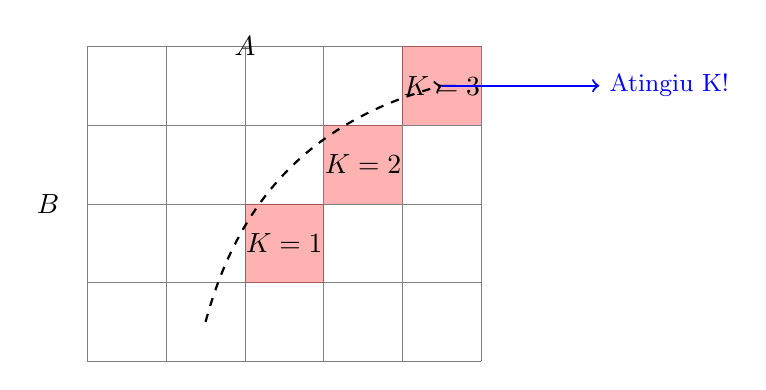
\begin{tikzpicture}
    % Diagrama ilustrativo do Grid de DP
    \draw[step=1cm,gray,very thin] (0,0) grid (5,4);
    
    % Destacando uma diagonal de match
    \fill[red, opacity=0.3] (2,1) rectangle (3,2);
    \fill[red, opacity=0.3] (3,2) rectangle (4,3);
    \fill[red, opacity=0.3] (4,3) rectangle (5,4);
    
    \node at (2.5, 1.5) {$K=1$};
    \node at (3.5, 2.5) {$K=2$};
    \node at (4.5, 3.5) {$K=3$};
    
    \draw[->, thick, blue] (4.5, 3.5) -- (6.5, 3.5) node[right] {\small Atingiu K!};
    \draw[->, thick, dashed, black] (1.5, 0.5) to[bend left] (4.5, 3.5);
    \node at (2, 4) {$A$};
    \node at (-0.5, 2) {$B$};
\end{tikzpicture}
\end{center}

\newpage

\section*{Fluxograma da Solução}

Abaixo ilustra-se as bifurcações de raciocínio a cada avanço no grid da DP.

\vspace{0.5cm}
\begin{center}
\begin{tikzpicture}[node distance=2.5cm, auto]
    \node [wokstart] (start) {Para $i=1..N$, $j=1..M$};
    \node [wokdecision, below of=start] (chars) {$A[i] == B[j]$?};
    
    \node [wokstep, right of=chars, node distance=5cm] (notmatch) {`match = 0`\\ dp herda bordas};
    \node [wokstep, below of=chars] (yesmatch) {`match = match[i-1][j-1] + 1`};
    
    \node [wokdecision, below of=yesmatch] (reachK) {`match $\ge K$`?};
    \node [wokstep, below of=reachK] (updatef) {Calcular nova $f$ e max $dp$};
    \node [wokend, below of=updatef] (end) {Salvar na célula e seguir};

    \draw [->] (start) -- (chars);
    \draw [->] (chars) -- node[midway, above] {Não} (notmatch);
    \draw [->] (chars) -- node[midway, left] {Sim} (yesmatch);
    \draw [->] (yesmatch) -- (reachK);
    
    \draw [->] (reachK) -- node[midway, left] {Sim} (updatef);
    \draw [->] (reachK) -- node[midway, right] {Não} (end);
    \draw [->] (notmatch) |- (end);
    \draw [->] (updatef) -- (end);
\end{tikzpicture}
\end{center}
\vspace{0.5cm}

\section*{Análise de Complexidade}

\begin{table}[h]
\centering
\begin{tabularx}{\textwidth}{|X|c|c|X|}
\hline
\textbf{Fase} & \textbf{Tempo} & \textbf{Espaço} & \textbf{Observação} \\
\hline
Alocação das Matrizes & $O(N^2)$ & $O(N^2)$ & Três matrizes de tamanho $N \times M$. Caso limite, pode-se economizar memória guardando só 2 linhas. \\
\hline
Travessia da Programação Dinâmica & $O(N^2)$ & $O(1)$ & Iteração dupla clássica onde cada par avaliado processa um limite fixo de comparações independentes do tamanho da string. \\
\hline
\textbf{Total} & \textbf{$O(N^2)$} & \textbf{$O(N^2)$} & Uma redução colossal frente ao $O(N^3)$, validando perfeitamente a barreira de 1 segundo de tempo de CPU. \\
\hline
\end{tabularx}
\end{table}

\newpage
\begin{notebox}
\textbf{Tutorial Recomendado:}
Para um profundo aprofundamento na família de problemas \textit{Longest Common Subsequence} e como aplicar transições avançadas envolvendo blocos lógicos contíguos (muito comum no ramo da Bioinformática, que estuda pareamento de sequências genômicas), consulte o clássico "Introduction to Algorithms" (Cormen, Leiserson, Rivest, Stein), capítulo 15 sobre Programação Dinâmica. Adicionalmente, treine outras restrições e topologias de grids no \textit{Competitive Programming 3} ou \textit{4}.
\end{notebox}

\vfill
\wokfooter{0275}{WOK}

\end{document}
